\chapter{Testing and practical application of text classification using software} \label{chapt3}
\section{Software selection} \label{sect3_1}

The most popular languages in data analysis area are Python and R.
Python3 language was chosen as more convenient for machine learning and beyond variety of libraries, including:

\begin{itemize}
	\item pandas
	\item sklearn
	\item gensim
	\item keras
	\item tensorflow
	\item matplotlib
	\item psycopg2
\end{itemize}

The prototyping of models were made in the separate Jupyter notebooks and then re-factored into 
project using the Python IDE for developers be JetBrains company - PyCharm. 
The server with  Intel(R) Core(TM) i7-4770 CPU @ 3.40GHz, 15 $\times$ 2 GB DDR3-1333 was used. 

As a word vectors representation I used pre-trained word vectors which were trained on Wikipedia using fastText technique by Facebook research team and shared to the community \cite{fasttext}. These vectors in dimension 300 were obtained using the skip-gram model with default parameters.

My main requirement for the framework for building deep neural network models were:
\begin{itemize}
	\item well described documentation
	\item simplicity of usage
	\item learning speed
	\item reliability
\end{itemize}

Among a wide range of frameworks which are available in open source: 
CNTK, Theano, MAXNET, Lasagne - Tensorflow framework was chosen. 
Tensorflow has a flexible architecture allows easy deployment of computation across a variety of platforms (CPUs, GPUs, TPUs). To speed up the experiments with architecture of NN, I switched to a high-level neural networks API, written in Python and capable of running on top of TensorFlow. 

\section{Dataset selection and exploration} \label{sect3_2}


\begin{table}[]
	\centering
	\caption{My caption}
	\label{my-label}
	\begin{tabular}{|l|l|l|l|}
		\hline
		\textbf{lvl1} & \textbf{lvl2} & \textbf{titles}                  & \textbf{descriptions}                                                                       \\ \hline
		6             & 29            & Clean Toyota Camry 2008 Silver   & Fairly used Toyota 08 Camry with no problems V4 engine fabric seats and interior            \\ \hline
		5             & 25            & Look Unique                      & Nice, quality, adorable,unique dress available now, whatsapp me                             \\ \hline
		6             & 29            & Mercedes Benz Ml 430 2001 Silver & mercedes benz ml430 , 2001 model in good condition , engine and gear box ok, ac , cd player \\ \hline
		5             & 25            & Versace Shirt Dress              & Adorable versace shirt dress, whatsapp me on \_large\_number\_                              \\ \hline
		5             & 25            & Addidas Jumpsuit                 & Nice quality addidas jumpsuit available, whatsapp me                                        \\ \hline
	\end{tabular}
\end{table}


\begin{table}[h]
	\centering
	\caption{Training set general information}
	\label{my-label}
	\begin{tabular}{|c|c|}
		\hline
	\textbf{	Number of variables     }      & 4      \\
		\hline
	\textbf{	Numeric variables}	 		  & 2		 \\
		\hline
	\textbf{	Categorical	variables} 		  & 2		 \\
		\hline
		\textbf{Number of observations }       & 1000000  \\
		\hline
		\textbf{Total Missing (\%) }           & 2.4\%    \\
		\hline
		\textbf{Total size in memory }         & 57.7 MiB \\
		\hline
		\textbf{Average record size in memory} & 48.0 B  \\
		\hline
	\end{tabular}
\end{table}

The total number of first level categories is 16.

\begin{table}[h]
	\centering
	\caption{Information about first level categories}
	\label{my-label}
	\begin{tabular}{|l|l|l|l|}
		\hline
	\textbf{Value }             & \textbf{Count}  & \textbf{Frequency} (\%) \\ \hline
		6                & 207695 & 20.8\%           \\ \hline
		5                & 184934 & 18.5\%           \\ \hline
		1                & 133135 & 13.3\%           \\ \hline
		4                & 97799  & 9.8\%            \\ \hline
		3                & 87574  & 8.8\%           \\ \hline
		110              & 60214  & 6.0\%            \\ \hline
		9                & 55459  & 5.5\%            \\ \hline
		27               & 52419  & 5.2\%            \\ \hline
		47               & 38985  & 3.9\%            \\ \hline
		140              & 36442  & 3.6\%           \\ \hline
		Other values (6) & 45344  & 4.5\%            \\ \hline
	\end{tabular}
\end{table}

The total number of second level categories is 182.

\begin{table}[h]
	\centering
	\caption{Information about second level categories}
	\label{my-label}
	\begin{tabular}{|l|l|l|}
		\hline
		\textbf{Value }             & \textbf{Count}  & \textbf{Frequency} (\%) \\ \hline
		29                 & 194714 & 19.5\%         \\ \hline
		14                 & 115471 & 11.5\%         \\ \hline
		55                 & 72050  & 7.2\%          \\ \hline
		25                 & 61308  & 6.1\%          \\ \hline
		16                 & 32719  & 3.3\%          \\ \hline
		20                 & 23298  & 2.3\%          \\ \hline
		169                & 18743  & 1.9\%          \\ \hline
		42                 & 18490  & 1.8\%          \\ \hline
		44                 & 17740  & 1.8\%          \\ \hline
		279                & 15544  & 1.6\%          \\ \hline
		Other values (172) & 429923 & 43.0\%         \\ \hline
	\end{tabular}
\end{table}


\begin{table}[h]
	\centering
	\caption{Information about categorical features}
	\label{my-label}
	\begin{tabular}{llll}
		\hline
\multicolumn{1}{|l|}{\textbf{Column}} & \multicolumn{1}{l|}{\textbf{Distinct count}} & \multicolumn{1}{l|}{\textbf{Unique (\%)}} & \multicolumn{1}{l|}{\textbf{Missing (\%)}} \\ \hline
		\multicolumn{1}{|l|}{titles}       & \multicolumn{1}{l|}{619948}         & \multicolumn{1}{l|}{62.0\%}      & \multicolumn{1}{l|}{0.00\%}       \\ \hline
		\multicolumn{1}{|l|}{descriptions} & \multicolumn{1}{l|}{869554}         & \multicolumn{1}{l|}{87.0\%}      & \multicolumn{1}{l|}{0.00\%}       \\ \hline
	\end{tabular}
\end{table}

\section{Data preparation} \label{sect3_3}

\begin{figure}[ht] 
	\center
	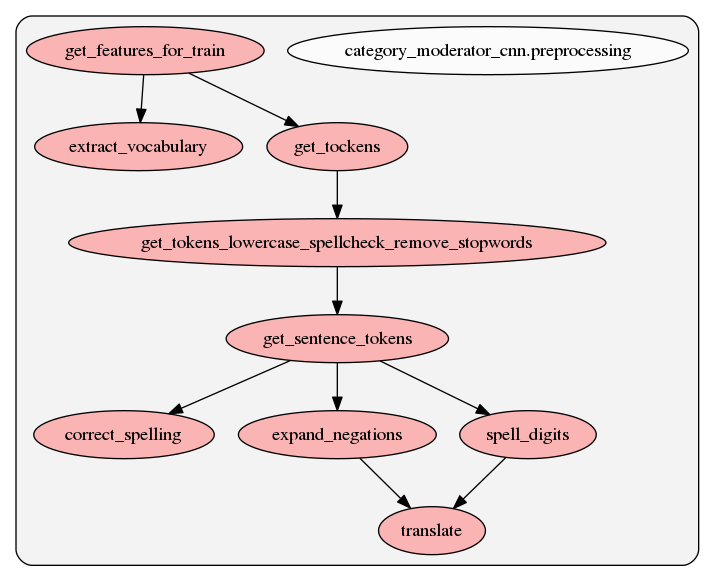
\includegraphics [scale=0.5] {p3_preprocessing.png}
	\label{img:p3_preprocessing}  
	\caption{The detailed internals of a LSTM} 
\end{figure}


\newcolumntype{b}{X}
\newcolumntype{s}{>{\hsize=.5\hsize}X}

\begin{table}[h]
	\centering
	\caption{Simplified event structure of data preprocessing}
	\label{my-label}
	\begin{tabulary}{1.0\textwidth}{|L|L|L|L|L|L}
		\hline
		\textbf{Functions}                                    & \textbf{Explanation}                                                                                                                \\ \hline
		get\_features\_for\_train                             & Unifying function which upload raw data and call nested functions                                                                   \\ \hline
		extract\_vocabulary                                   & form vocabulary from unique words                                                                                                   \\ \hline
		get\_tokens                                           & Parallel batch execution of texts preprocessing which save and return preprocessed tokens for both test and train.                  \\ \hline
		get\_tokens\_lowercase\_spellcheck\_remove\_stopwords & wrap over get\_sentence\_tokens which set necessary flags for it                                                                    \\ \hline
		get\_sentence\_tokens                                 & recieves single sentence breaks it into tokens, make all of them to lowercase, correct spelling mistakes and replace specific words \\ \hline
		correct\_spelling                                     & Correct spelling mistakes using dictionary with around 15000 most common mistakes                                                   \\ \hline
		expand\_negations                                     & replace mobile phones, dates, prices, and common abbreviation with specific words such as \_year\_, price,  \_large\_number\_ etc.  \\ \hline
		spell\_digits                                         & single digits are replaced with corresponding word 1 $\rightarrow$ one …                                                                          \\ \hline
		translate                                             & function which makes replacement of words                                                                                           \\ \hline
	\end{tabulary}
\end{table}

